\chapter{Πειράματα και Αποτελέσματα}

Στο κεφάλαιο αυτό θα αναλύσουμε τα πειράματα που έγιναν για την εκπαίδευση του μοντέλου παραγωγής κώδικα και θα μελετήσουμε την ποιότητα του παραγόμενου κώδικα.
Θα εξετάσουμε ξεχωριστά κάθε σετ δεδομένων και θα συγκρίνουμε τις επιλογές και τις επιδόσεις των δύο προσεγγίσεων σε καθ' ένα από αυτά.

\section{Πειράματα Eκπαίδευσης}

Ένα πολύ σημαντικό κομμάτι της εκπαίδευσης ενός τέτοιου συστήματος είναι η κατάλληλη επιλογή των υπερ-παραμέτρων.
Αποδεικνύεται πως η αποδοτικότερη μέθοδος για την επιλογή τους είναι η τυχαία μέθοδος αναζήτησης \cite{Bergstra2012}.
Η υπολογιστική πολυπλοκότητα που εισάγουν τα αναδραστικά νευρωνικά δίκτυα και οι περιορισμένοι υπολογιστικοί πόροι που είχαμε στη διάθεση μας κάνουν την τυχαία μέθοδο εξαιρετικά χρονοβόρα διαδικασία.
Αντ' αυτού επιλέγουμε εμπειρικά τις υπερ-παραμέτρους (με δοκιμές) και με οδηγό της επιλογές στη σύγχρονη σχετική βιβλιογραφία.

Η αναζήτηση των υπερ-παραμέτρων ξεκίνησε με βάση την πρωτότυπη υλοποίηση του \en{char-rnn}.
Αυτή χρησιμοποιεί μέγεθος \en{LSTM} ίσο με 512 και μήκος ακολουθίας ίσο με 50. Βάσει αυτής αναζητούμε το κατάλληλο μέγεθος παρτίδας, ρυθμό εκμάθησης και την πιθανότητα \en{dropout}.
Μετά από δοκιμές, τα καλύτερα αποτελέσματα στο σετ επιβεβαίωσης προκύπτουν για μέγεθος \en{LSTM} 200, ρυθμό εκμάθησης 0.02 και 20\% πιθανότητα \en{dropout}.
Τα τελικά μοντέλα επιλέγουμε να είναι μεγαλύτερα σε μέγεθος, επειδή καθ' όλη τη διάρκεια των δοκιμών παρουσιάζεται σημαντικό \en{underfitting}.
Η διακοπή της εκπαίδευσης γίνεται με τη μέθοδο \en{\textit{early stopping}}.
Σημειώνεται πως οι επιλεγμένες παράμετροι μπορεί να ευνοούν το μοντέλο \en{char-rnn} λόγω των παραπάνω αποφάσεων.
Η εξαντλητική αναζήτηση των υπερ-παραμέτρων με τη μέθοδο τυχαίας αναζήτησης όμως, θα διαρκούσε τουλάχιστον λίγους μήνες οπότε και δεν τη χρησιμοποιούμε.

\subsection{Πειράματα με τα 100 Δημοφιλέστερα \en{Github JavaScript Projects}}

Το σετ δεδομένων αυτό αποτελείται από τα 100 πιο δημοφιλή \en{projects} σε γλώσσα \en{JavaScript} στον ιστότοπο αποθετηρίων λογισμικού \en{github}\footnote{\en{\url{www.github.com}}}.
Μετά το \en{preprocessing} παίρνουμε ακολουθίες συνολικού μήκους περίπου 79 εκατομμυρίων χαρακτήρων.
Υπάρχουν 212 διαφορετικοί χαρακτήρες, συμπεριλαμβανομένων των ειδικών χαρακτήρων αρχής και τέλους αρχείων.
Χρησιμοποιούμε το 95\% των δεδομένων για την εκπαίδευση του συστήματος και το υπόλοιπο 5\% για την επικύρωση της μάθησης.
Λόγω της έλλειψης τεστ σετ δεν εξασφαλίζεται πως τα αποτελέσματα μας δεν κάνουν \en{overfit} στα δεδομένα επικύρωσης. Αυτό όμως είναι δευτερευούσης σημασίας αφού στόχος μας είναι να παράγουμε κώδικα και δεν υπάρχουν διαθέσιμα συγκριτικά αποτελέσματα (\en{benchmark results}) για τον σκοπό αυτό.

Η στρατηγική επιλογής των παραμέτρων έχει ως εξής: Για να είναι οι δύο προσεγγίσεις συγκρίσιμες κρατάμε ίδιο το μέγεθος των κρυφών επιπέδων.
Από αυτή την επιλογή εξαρτάται κυρίως ο αριθμός συνολικών παραμέτρων προς εκπαίδευση.
Για το πρώτο σετ δεδομένων αποφασίζουμε τον αριθμό αυτό σε 1024, αριθμός αρκετά μεγάλος ώστε να είναι αντιμετωπίσιμο από το σύστημα το ογκώδες σετ δεδομένων.

Η επόμενη υπερ-παράμετρος που πρέπει να αποφασιστεί είναι το μήκος της εκπαιδευτικής ακολουθίας, η μεταβλητή $k_2$ του αλγορίθμου \en{TBPTT}.
Η υπερ-παράμετρος αυτή έχει μεγάλη σχέση τόσο με την ποιότητα του παραγόμενου κώδικα, αφού ελέγχει πόσους από τους προηγούμενους χαρακτήρες <<βλέπει>> το σύστημα, αλλά και με τον χρόνο εκτέλεσης μιας εποχής, αφού μεγαλύτερες ακολουθίες εισάγουν υπολογιστική πολυπλοκότητα.
Το μέγεθος των εκπαιδευτικών ακολουθιών αποφασίζεται στους 100 χαρακτήρες και για τα δύο μοντέλα.

Ο ρυθμός εκμάθησης είναι άμεσα συνδεδεμένος με το μέγεθος παρτίδας.
Όσο περισσότερα παραδείγματα βλέπει ταυτόχρονα το σύστημα τόσο πιο σίγουρο θα πρέπει να είναι για τα συμπεράσματα του.
Εξαγωγή δυνατών συμπερασμάτων από λιγοστά παραδείγματα πρέπει να αποφεύγεται.
Τελικώς δείχνουμε 200 ακολουθίες σε κάθε βήμα εκμάθησης και θέτουμε τον ρυθμό εκμάθησης στην τιμή 0.002, ώστε να γεμίζουμε όσο καλύτερα γίνεται την μνήμη του υπολογιστικού συστήματος αλλά ταυτόχρονα να συνεχίσουμε να μαθαίνουμε αποτελεσματικά.
Σημειώνεται πως η προτεινόμενη τιμή για τον ρυθμό εκμάθησης της \en{rmsprop} είναι το 0.001.

Τέλος, επειδή το σετ δεδομένων  είναι αρκετά ογκώδες και περίπλοκο, είναι δύσκολο το μοντέλο μας να κάνει \en{overfit}. Έτσι, δε χρειάζεται η πιθανότητα \en{dropout} να είναι εξαιρετικά μεγάλη.
Επιλέγουμε την υπερ-παράμετρο αυτή στο 20\%, ενώ η γενική προτεινόμενη τιμή είναι 40\% με 50\%.
Ο αριθμός των εποχών αποφασίζεται έτσι ώστε κανένα από τα 2 μοντέλα να μη βελτιώνει τις επιδόσεις του στο σετ δεδομένων επιβεβαίωσης.
Ο αριθμός αυτός προκύπτει στις 60 εποχές.
Στον πίνακα \ref{hyper1} παρουσιάζονται συνοπτικά οι παραπάνω αποφάσεις.

\begin{table}[]
\centering
\caption{Υπερ-παράμετοι για τα 100 δημοφιλέστερα \en{Github js projects}}
\begin{tabularx}{\textwidth}{|X|X|X|}
\hline
                    & \en{char-rnn} & \en{labeled-char-rnn} \\
\hline
\en{\#} Παραμέτρων       & 23Μ             & 23Μ                     \\
\hline
\en{\#} Χαρακτήρων       & 212             & 212, 8                  \\
\hline
\en{\#} Εποχών       & 40             & 60                  \\
\hline
Μέγεθος \en{LSTM}  & 1024            & 1024                    \\
\hline
Μήκος Ακολουθίας    & 100             & 100                     \\
\hline
Ρυθμός Εκμάθησης    & 0.002           & 0.002                   \\
\hline
\% \en{Dropout}     & 20              & 20                      \\
\hline
Μέγεθος Παρτίδας    & 200             & 200                     \\
\hline
\end{tabularx}
\label{hyper1}
\end{table}

Η εκπαίδευση έγινε σε μία κάρτα γραφικών \en{Nvidia Gtx 960} με 4 \en{gb RAM} με τη βοήθεια της βιβλιοθήκης \en{keras}\footnote{\en{\url{https://keras.io}}}.
Η εκπαίδευση διαρκεί 6 περίπου ημέρες για το πρώτο μοντέλο και 7 περίπου για το δεύτερο.
Όπως αναφέραμε, η παρακολούθηση των επιδόσεων και η επιλογή των σετ βαρών για την παραγωγή κώδικα γίνεται σύμφωνα με την μετρική \en{average cross entropy per minibatch}.
Σημειώνεται πως η σύγκριση των μοντέλων στην μετρική αυτή γίνεται μόνο στο κομμάτι που αφορά την πρόβλεψη χαρακτήρων.
Στην εικόνα \ref{training1} φαίνεται η εξέλιξη της εκπαίδευσης των 2 μοντέλων στην περίοδο 40 και 60 εποχών στο σετ εκπαίδευσης και το σετ επαλήθευσης. 
%TODO Διάγραμμα training me σχόλια περι overfittinh και τετοια και επιλογής μοντέλο και ξαναγραψιμο της μετρικής που χρησιμοποιείται 1 + 0.2. Σχολιασμός των accuracy
Ως μοντέλα παραγωγής, επιλέγουμε αυτά με τα βάρη τις 38ης εποχής για το μοντέλο \en{char-rnn} και της 53ης εποχής για το μοντέλο \en{labeled-char-rnn}. Οι επιδόσεις τους συνοψίζονται στον πίνακα \ref{github-results}.
Τα αποτελέσματα της εκπαιδευτικής διαδικασίας είναι σε πρώτη όψη ικανοποιητικά. Οι καμπύλες εκπαίδευσης και επαλήθευσης μένουν σε κοντινά επίπεδα και για τα δύο μοντέλα, γεγονός που μαρτυρά καλή γενίκευση των χαρακτηριστικών που μαθαίνονται. Η ευστοχία, ιδιαίτερα, της ανάθεσης είδους στον επόμενο χαρακτήρα κυμαίνεται σε πολύ υψηλά επίπεδα. 

\begin{figure}[!htp]

	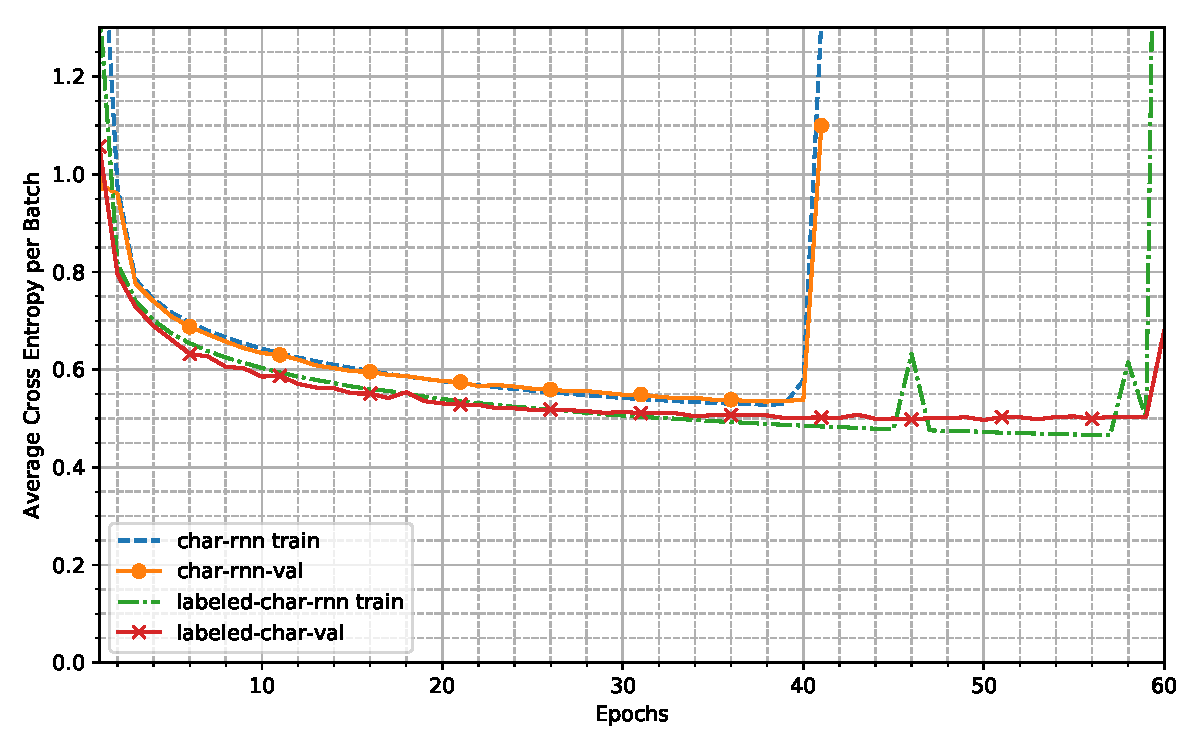
\includegraphics[trim = 2 2 2 2, clip, keepaspectratio, width=\textwidth]{images/training1.pdf}
	\centering
	\caption{Καμπύλες εκμάθησης για τα 100 δημοφιλέστερα \en{Github JavaScript projects}}
	\label{training1}
\end{figure}

\begin{table}
\centering
\caption{Επιλεγμένα μοντέλα}
\begin{tabularx}{\textwidth}{|l|X|X|X|}
\hline
                    & Εποχή & Λάθος Επιβεβαίωσης & \% Ευστοχίας\\
\hline
\en{char-rnn}       & 38             & 0.534    	& 85.6                \\
\hline
\en{labeled-char-rnn}       & 53 & 0.526, 0.11  	 & 87.2, 97.1      \\
\hline
\end{tabularx}
\label{github-results}
\end{table}

\subsection{Πειράματα με τα 200 Δημοφιλέστερα \en{npm JavaScript Projects}}

Το δεύτερο σετ δεδομένων αποτελείται από τις 200 πιο δημοφιλείς βιβλιοθήκες \en{javascript} του ιστοχώρου \en{www.npmjs.com}.
Οι ακολουθίες μετά την προ-επεξεργασία αριθμούν περίπου 49 εκατομμύρια χαρακτήρες με 210 διαφορετικούς χαρακτήρες. 
Σε αυτό το πείραμα χωρίζουμε το 90\% των ακολουθιών στο σετ εκπαίδευσης και το 10\% στο σετ επαλήθευσης, επειδή έχουμε λιγότερα δεδομένα και θέλουμε να αποφύγουμε μεγάλη διακύμανση στο σετ επαλήθευσης.

Οι αποφάσεις των υπερ-παραμέτρων βασίζονται στις παρατηρήσεις μας από τα προηγούμενα πειράματα. Έτσι, κρατάμε ίδιο το μέγεθος παρτίδας, τον ρυθμό εκμάθησης και το μήκος ακολουθίας.
Το σετ εκπαίδευσης έχει μικρότερο μέγεθος από το προηγούμενο πείραμα και από τις πρώτες δοκιμές παρατηρούμε σημαντικό \en{overfitting}.
Προς την κατεύθυνση καλύτερης γενίκευσης των συμπερασμάτων του συστήματος, αρχικά μικραίνουμε το δίκτυο θέτοντας το μέγεθος \en{LSTM} se 512, κίνηση η οποία μειώνει σημαντικά τις εκπαιδεύσιμες παραμέτρους του συστήματος.
Έπειτα αυξάνουμε την πιθανότητα \en{dropout} σε 30\% και 40\% που αποτέλεσμα έχει την αργότερη εκπαίδευση του αναδραστικού νευρωνικού δικτύου.
Για να αποζημιώσουμε την τελευταία μας επιλογή αυξάνουμε τις εκπαιδευτικές εποχές των μοντέλων στις 80.
Οι εκπαιδευτικές επιλογές συνοψίζονται στον πίνακα \ref{hyper2}.

\begin{table}
\centering
\caption{Υπερ-παράμετοι για τα \en{200} δημοφιλέστερα \en{npm js projects}}
\begin{tabularx}{\textwidth}{|X|X|X|}
\hline
                    & \en{char-rnn} & \en{labeled-char-rnn} \\
\hline
\en{\#} Παραμέτρων       & 10M             & 10M                     \\
\hline
\en{\#} Χαρακτήρων       & 210             & 210, 8                  \\
\hline
\en{\#} Εποχών       & 80             & 80                  \\
\hline
Μέγεθος \en{LSTM}  & 512            & 512                    \\
\hline
Μήκος Ακολουθίας    & 100             & 100                     \\
\hline
Ρυθμός Εκμάθησης    & 0.002           & 0.002                   \\
\hline
\% \en{Dropout}     & 30              & 40                      \\
\hline
Μέγεθος Παρτίδας    & 200             & 200                     \\
\hline
\end{tabularx}
\label{hyper2}
\end{table}

Η διαδικασία που ακολουθείται είναι η ίδια με του προηγούμενου πειράματος, δηλαδή εκπαιδεύουμε το σύστημα σε μία κάρτα γραφικών \en{Nvidia Gtx 960} με 4 \en{gb RAM} και επιλέγουμε το μοντέλο με τις καλύτερες επιδόσεις στη μετρική πρόβλεψης χαρακτήρων.
Η εκπαίδευση του \en{char-rnn} διαρκεί 3 ημέρες ενώ του \en{labeled-char-rnn} διαρκεί περίπου 4. Η εξέλιξη της εκπαίδευσης φαίνεται στην εικόνα \ref{training2}.

\begin{figure}
	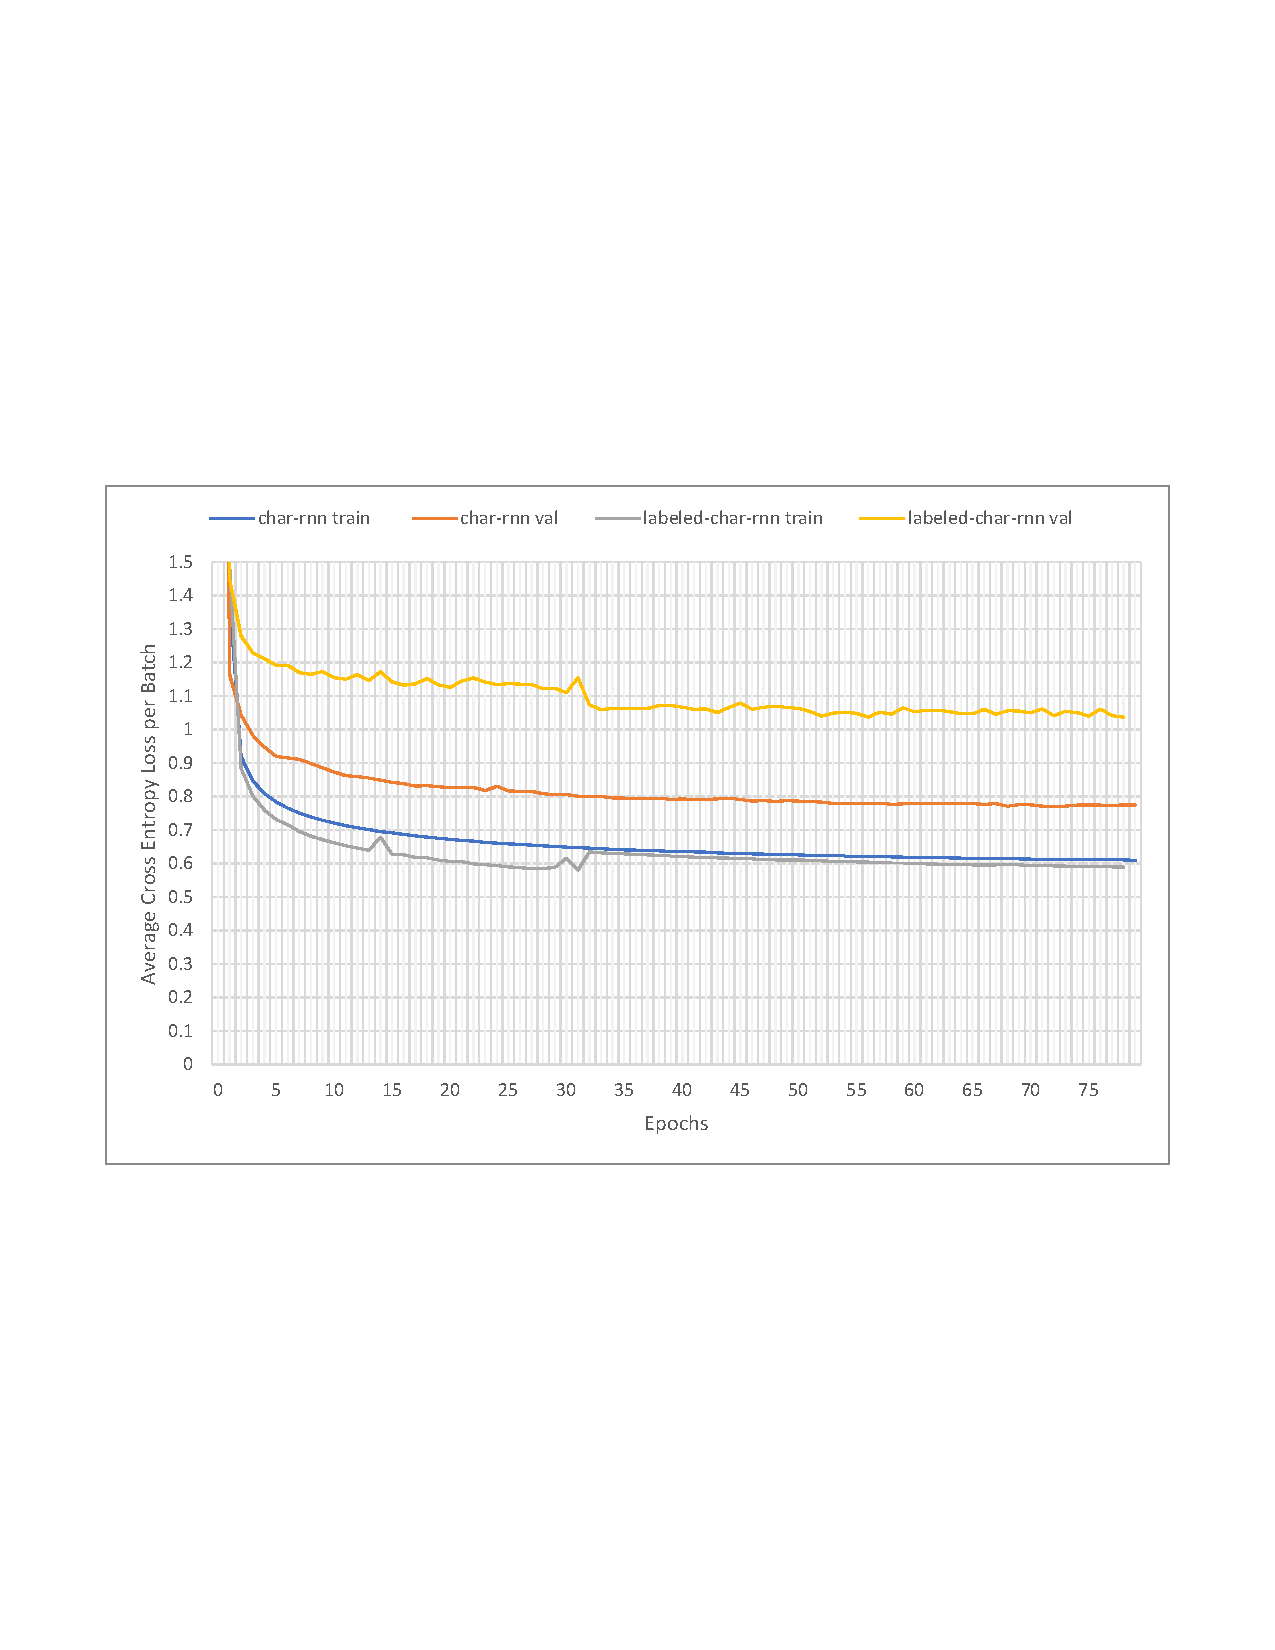
\includegraphics[width=\textwidth, trim = 2 2 2 2, clip, keepaspectratio]{images/training2.pdf}
	\centering
		\caption{Καμπύλες εκμάθησης για τα 200 δημοφιλέστερα \en{npm JavaScript projects}}
	\label{training2}
\end{figure}


Το επιλεγόμενο μοντέλο για το \en{char-rnn} είναι αυτό της 72ης εποχής  και για το \en{labeled-char-rnn} το επιλεγόμενο μοντέλο είναι αυτό της 78ης εποχής. Τα αποτελέσματα συνοψίζονται στον πίνακα \ref{npm-results}. Είναι εμφανές από το διάγραμμα ότι τα μοντέλα μας δυσκολεύονται περισσότερο να γενικεύσουν τα συμπεράσματα που εξάγουν από αυτό το σετ δεδομένων. Η ικανότητα πρόβλεψης του είδους του επόμενου χαρακτήρα παραμένει σε σχετικά υψηλά επίπεδα αλλά η προσθήκη της δεν βελτιώνει τις επιδόσεις στο σετ επιβεβαίωσης. Θα εξετάσουμε αναλυτικότερα τα αποτελέσματα αυτά στο υποκεφάλαιο των αποτελεσμάτων και στο κεφάλαιο των συμπερασμάτων.

\begin{table}
\centering
\caption{Επιλεγμένα μοντέλα}
\begin{tabularx}{\textwidth}{|l|X|X|X|}
\hline
                    & Εποχή & Λάθος Επιβεβαίωσης & \% Ευστοχίας\\
\hline
\en{char-rnn}       & 72             &  0.771   	& 78.9                \\
\hline
\en{labeled-char-rnn}       & 78 & 1.038, 0.161  	 & 72.3, 94.7      \\
\hline
\end{tabularx}
\label{npm-results}
\end{table}


\section{Αποτελέσματα}

Χρησιμοποιούμε τα μοντέλα που εκπαιδεύτηκαν παραπάνω για να παράξουμε 100 αρχεία κώδικα για κάθε προσέγγιση και κάθε ομάδα μοντέλων.
Επιλέγουμε ένα \en{JavaScript project} με το οποίο αρχικοποιούμε κάθε ομάδα μοντέλων. 
Η αρχικοποίηση του μοντέλου γίνεται με σκοπό την έμμεση οδήγηση του.
Αρχικά θα εξετάσουμε την ποιότητα του κώδικα εποπτικά και έπειτα θα χρησιμοποιήσουμε το εργαλείο \en{\textit{jshint}}\footnote{\en{\url{http://jshint.com}}} για να κάνουμε στατική ανάλυση του κώδικα.

\subsection{Παραγόμενος Κώδικας στα 100 Δημοφιλέστερα \en{Github Javascript Projects}}

Επιλέγουμε ένα \en{project} που δεν έχει εμφανιστεί στη διάρκεια της εκπαίδευσης και της επαλήθευσης.
Συγκεκριμένα επιλέγουμε το \en{hyper terminal} που είναι το πιο δημοφιλές \en{JavaScript project} στο \en{github} το πρώτο εξάμηνο του 2017.
Ο κώδικας 5.1 είναι ένα αρχείο από το \en{project} αυτό.

\selectlanguage{english}
\lstinputlisting[language=JavaScript, caption={\tg{Δείγμα κώδικα απο το }\en{hyper terminal}}]{code/hyper.js}
\selectlanguage{greek}

Οι κώδικες 5.2, 5.3 είναι δημιουργήματα των μοντέλων \en{char-rnn} και \en{labeled-char-rnn} αντίστοιχα. Τα αρχεία αυτά επιλέχτηκαν χάρη στο μικρό μέγεθός τους και την συντακτική ορθότητα.

Ήδη εποπτικά παρατηρούμε τη δυνατότητα και των δύο μοντέλων να αναπαράγουν συντακτικές δομές, όπως οι παρενθέσεις και οι αγκύλες, αλλά και λογικές, όπως οι συναρτήσεις και οι δομές πολλαπλών επιλογών.
Φαινομενικά αυτό είναι ένα συνηθισμένο αρχείο \en{javascript}.
Με μία δεύτερη, αναλυτικότερη ματιά παρατηρούμε σημαντικά λάθη στη χρήση μη ορισμένων μεταβλητών (5.2, γραμμή 3), την ύπαρξη γραμματικών λαθών (5.2, γραμμή 23) και ενέργειες χωρίς αποτέλεσμα (5.2, γραμμή 21). 
Είναι εύκολο να συμπεράνει κανείς, ίσως και χωρίς να είναι γνώστης της γλώσσας, πως τα προγράμματα αυτά δεν θα καταφέρουν να μεταφραστούν.
\pagebreak

\selectlanguage{english}
\lstinputlisting[language=JavaScript, caption={\tg{Δείγμα κώδικα από το }\en{char-rnn}}]{code/charrnnGithub.js}
\selectlanguage{greek}
 
Για την καλύτερη εκτίμηση των αποτελεσμάτων των νευρωνικών δικτύων, και για τη σύγκριση των δύο  θα ακολουθήσουμε μια πιο ποσοτική προσέγγιση. 
Με τη χρήση του εργαλείου ανάλυσης κώδικα \en{\textit{jshint}} θα εξετάσουμε τον αριθμό των συντακτικών και διαφόρων άλλων λαθών \en{(Errors)} που εντοπίζονται και μέχρι πιο σημείο καταφέρνουν να αναγνωστούν πριν βρεθεί ένα ανεπανόρθωτο συντακτικό λάθος (\en{\% Scanned Lines}).
Σημειώνεται πως τα μοντέλα αποφασίζουν αυτόνομα το μήκος του κώδικα, με τη χρήση των ειδικών χαρακτήρων, αλλά τίθεται ένα άνω όριο 15000 χαρακτήρων στο οποίο θεωρούμε ότι το αρχείο ξεφεύγει διαχειρισιμότητας λόγω μεγέθους.
Στις εικόνες \ref{static-github-char} - \ref{MCE2-githubLabeled} φαίνονται τα αποτελέσματα της παραπάνω ανάλυσης και το μήκος των παραγόμενων αρχείων.

\newpage
\selectlanguage{english}
\lstinputlisting[language=JavaScript, caption={\tg{Δείγμα κώδικα από το }\en{labeled-char-rnn}}]{code/labeledcharrnnGithub.js}
\selectlanguage{greek}

\begin{figure}[!htb]
	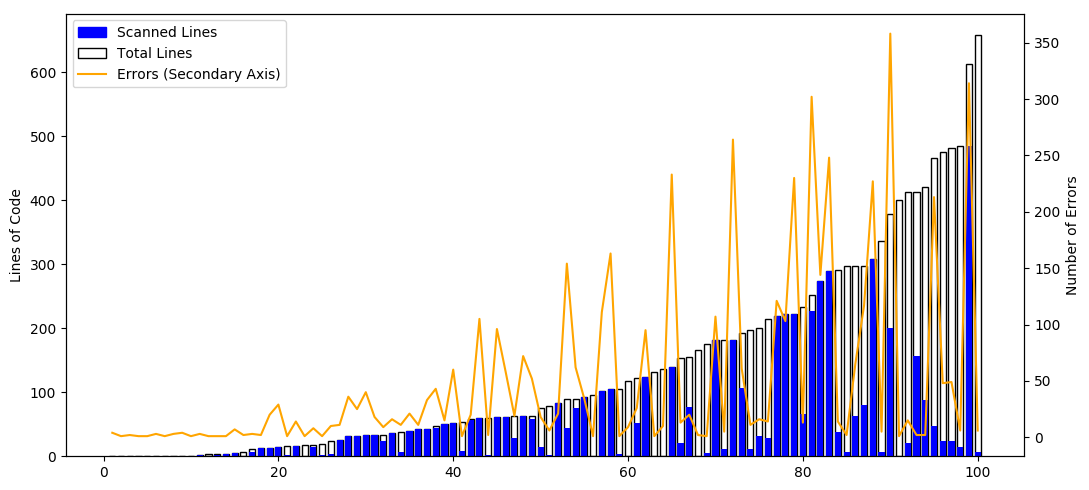
\includegraphics[width=\textwidth, keepaspectratio]{images/jshint-githubChar.png}
	\caption{Στατική ανάλυση κώδικα για τα αποτελέσματα του \en{char-rnn} μοντέλου}
	\label{static-github-char}
\end{figure}

\begin{figure}[!htb]
	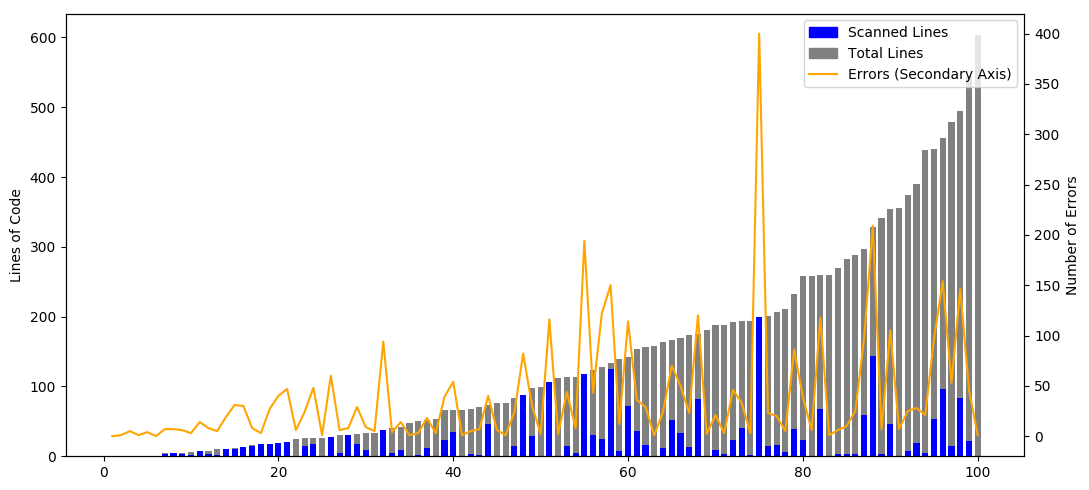
\includegraphics[width=\textwidth, keepaspectratio]{images/jshint-githubLabeled.png}
	\caption{Στατική ανάλυση κώδικα για τα αποτελέσματα του \en{labeled-char-rnn} μοντέλου}
	\label{static-github-labeled}
\end{figure}

\begin{figure}[!htb]
	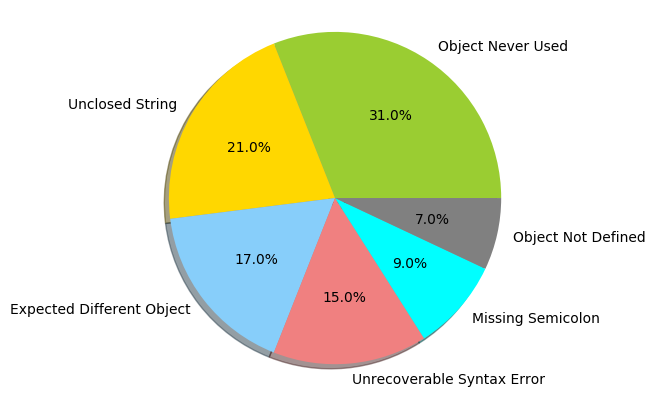
\includegraphics[width=\textwidth, keepaspectratio]{images/MCE-githubchar.png}
	\caption{Συνηθέστερο λάθος των αρχείων του \en{char-rnn}}
	\label{MCE1-githubchar}
\end{figure}

\begin{figure}[!htb]
	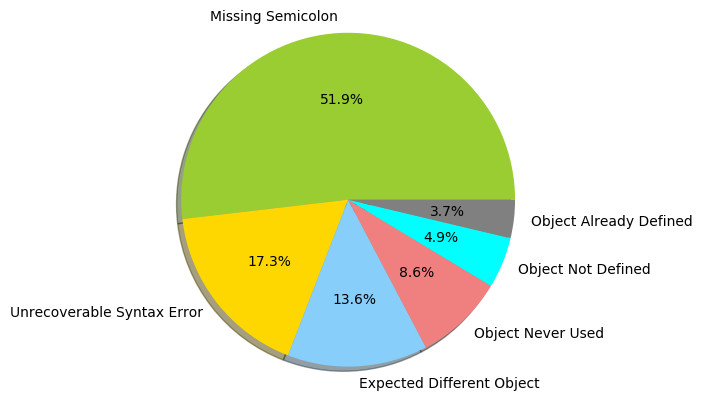
\includegraphics[width=\textwidth, keepaspectratio]{images/MCE2-githubchar.png}
	\caption{Δεύτερο συνηθέστερο λάθος των αρχείων του \en{char-rnn}}
	\label{MCE2-githubchar}
\end{figure}

\begin{figure}[!htb]
	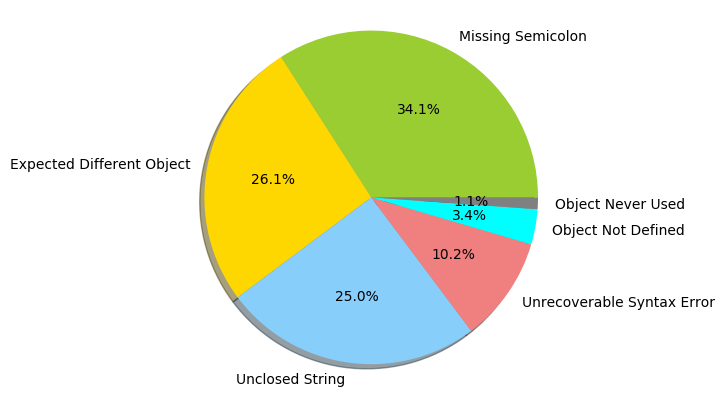
\includegraphics[width=\textwidth, keepaspectratio]{images/MCE-githubLabeled.png}
	\caption{Συνηθέστερο λάθος των αρχείων του \en{labeled-char-rnn}}
	\label{MCE1-githubLabeled}
\end{figure}

\begin{figure}[!htb]
	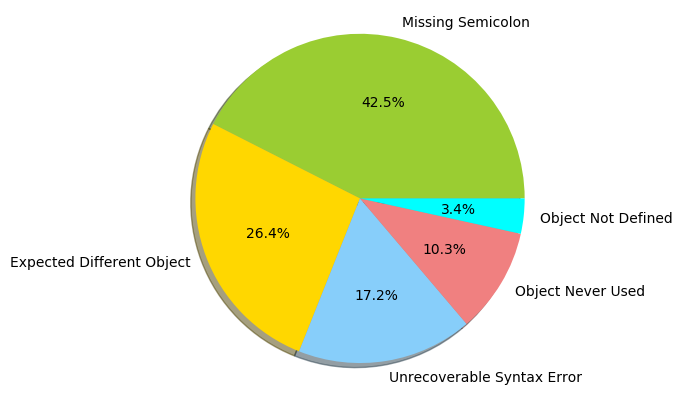
\includegraphics[width=\textwidth, keepaspectratio]{images/MCE2-githubLabeled.png}
	\caption{Δεύτερο συνηθέστερο λάθος των αρχείων του \en{labeled-char-rnn}}
	\label{MCE2-githubLabeled}
\end{figure}

Στα σχήματα \ref{static-github-char} και \ref{static-github-labeled} μπορούμε να συγκρίνουμε τις επιδόσεις των δύο μοντέλων.
Τα στατιστικά των 100 αρχείων έχουν ταξινομηθεί κατά τον αύξοντα αριθμό γραμμών.
Αρχικά παρατηρούμε πως και τα δύο μοντέλα παράγουν κάποια κενά αρχεία ή αρχεία με 1 ή 2 γραμμές.
Το μέσο μήκος των αρχείων είναι αρκετά κοντινό (137 γραμμές \en{char-rnn} -- 142 γραμμές \en{labeled-char-rnn}) και το δεύτερο μοντέλο καταφέρνει να κλείσει τα αρχεία σε λιγότερο από 15000 χαρακτήρες 9\% των περιπτώσεων ενώ το πρώτο 6\%.
Αν και το \en{labeled-char-rnn} έχει περισσότερη πληροφορία για τον κώδικα, παράγει αρχεία που ολοκληρώνουν την ανάλυση κώδικα με αρκετά μικρότερη συχνότητα.
Η γενική εικόνα που παίρνουμε από την ανάλυση αυτή είναι απογοητευτική για το δεύτερο μοντέλο, που ενώ έχει \en{a priori} γνώση για τη γλώσσα αποτυγχάνει να την αποτυπώσει με τρόπο που να παράγει ποιοτικά αποτελέσματα.

Τα είδη των συνηθέστερων λαθών μαρτυρούν τις αδυναμίες της προσέγγισης μας στην παραγωγή κώδικα.
Ακόμα και αν καταφέρνουν να δημιουργηθούν μικρά κομμάτια λειτουργικού κώδικα η έλλειψη ανεξάρτητης μνήμης και η στοχαστική φύση της παραγωγής δυσκολεύουν τα μοντέλα ως προς τη διαχείριση των διαφόρων μεταβλητών, τη χρήση της σύνταξης και τη επίτευξη του τελικού σκοπού.
Αυτή είναι η κύρια αιτία των λαθών \en{Object Already Defined, Object Not Defined, Object Never Used, Expected Different Object}.
Αρκετά συχνά η δημιουργία αλφαριθμητικών ξεφεύγει της διαχείρισης του μοντέλου και συνεχίζεται να γράφεται κώδικας μέσα σε κάποιο αλφαριθμητικό - που είναι ο κύριος λόγος της ύπαρξης του \en{Unclosed String} σε συνδυασμό με το \en{Missing Semicolon}.

\subsection{Παραγόμενος Κώδικας στα 200 Δημοφιλέστερα \en{npm JavaScript Projects}}

Ακολουθούμε ανάλυση όμοια με την προηγούμενη υπο-ενότητα.
Το \en{project} αρχικοποίησης που χρησιμοποιείται είναι το \en{lodash}, μια βιβλιοθήκη της \en{JavaScript} που διευκολύνει τη διαχείριση διανυσμάτων, αντικειμένων και αλφαριθμητικών . Ο κώδικας 5.4 είναι του ιδίου \en{project} και οι κώδικες 5.5, 5.6 είναι επιλεγμένοι κώδικες των παραγόμενων μοντέλων. 
%\pagebreak

\newpage
\selectlanguage{english}
\lstinputlisting[language=JavaScript, caption={\tg{Δείγμα κώδικα απο το }\en{lodash}}]{code/lodash.js}
\selectlanguage{greek}

\selectlanguage{english}
\lstinputlisting[language=JavaScript, caption={\tg{Δείγμα κώδικα απο το }\en{char-rnn}}]{code/charnpm.js}
\selectlanguage{greek}

\pagebreak

\selectlanguage{english}
\lstinputlisting[language=JavaScript, caption={\tg{Δείγμα κώδικα απο το }\en{labeled-char-rnn}}]{code/npmLabel.js}
\selectlanguage{greek}

Στα σχήματα \ref{static-npm-char} και \ref{static-npm-labeled} μπορούμε να συγκρίνουμε τις επιδόσεις των δύο μοντέλων.
To \en{dataset} αυτό περιέχει κατά μέσο όρο μικρότερα αρχεία οπότε και τα μεγέθη των παραγόμενων αρχείων είναι μικρότερα (113 γραμμές \en{char-rnn} -- 47 γραμμές \en{labeled-char-rnn}). 
Και πάλι, το \en{labeled-char-rnn} μοντέλο κλείνει με μεγαλύτερη συνέπεια τα αρχεία του.
Τα ποσοστά ολοκλήρωσης της συντακτικής ανάλυσης και οι μέσοι όροι λαθών δείχνουν βελτίωση σε σχέση με το προηγούμενο σετ δεδομένων, ενώ τα παρόντα μοντέλα χρησιμοποιούν σημαντικά λιγότερες παραμέτρους.
Ωστόσο, και σε αυτό το πείραμα το \en{labeled-char-rnn} μοντέλο αδυνατεί να χρησιμοποιήσει την παραπάνω πληροφορία που του δίνεται. Τα μοτίβα των συνηθισμένων λαθών επαναλαμβάνονται (\ref{MCE1-npmchar} - \ref{MCE2-npmlabeled})

\begin{figure}
	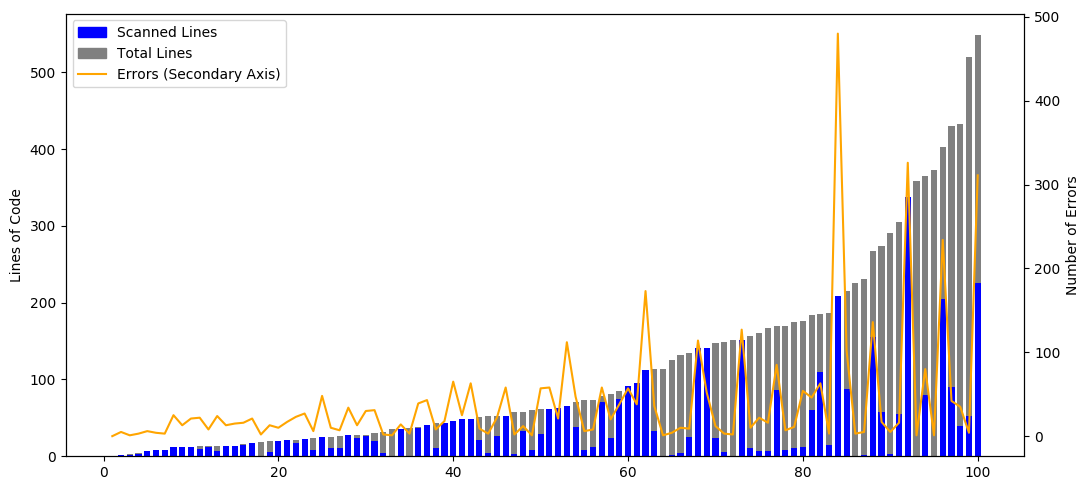
\includegraphics[width=\textwidth, keepaspectratio]{images/jshint-npmchar.png}
	\caption{Στατική ανάλυση κώδικα για τα αποτελέσματα του \en{char-rnn} μοντέλου}
	\label{static-npm-char}
\end{figure}

\begin{figure}
	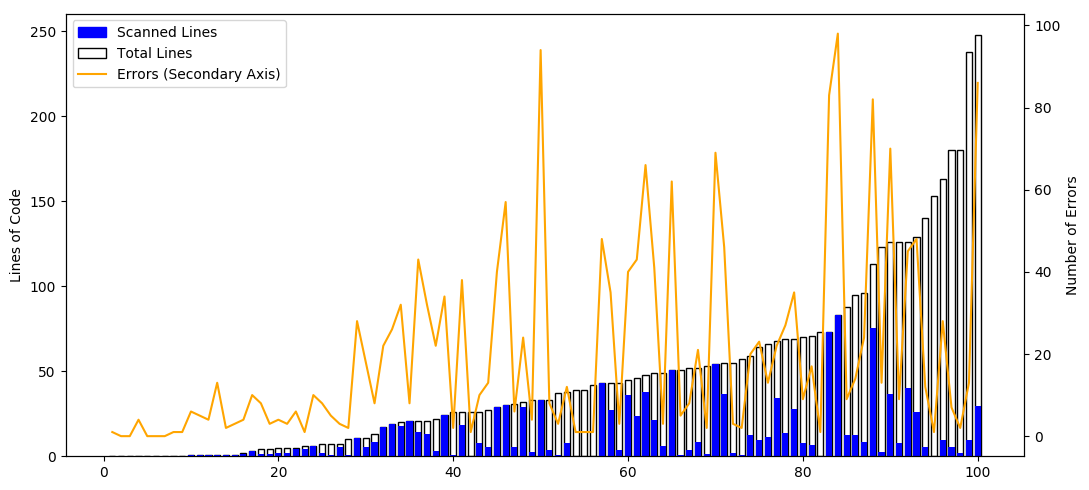
\includegraphics[width=\textwidth, keepaspectratio]{images/jshint-npmlabeled.png}
	\caption{Στατική ανάλυση κώδικα για τα αποτελέσματα του \en{labeled-char-rnn} μοντέλου}
	\label{static-npm-labeled}
\end{figure}

\begin{figure}
	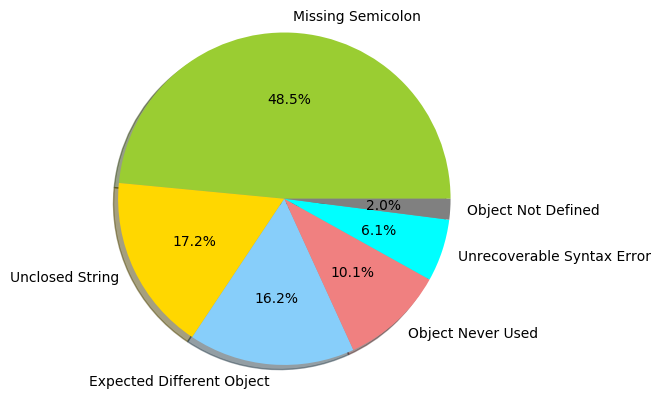
\includegraphics[width=\textwidth, keepaspectratio]{images/MCE-npmchar.png}
	\caption{Συνηθέστερο λάθος των αρχείων του \en{char-rnn}}
	\label{MCE1-npmchar}
\end{figure}

\begin{figure}
	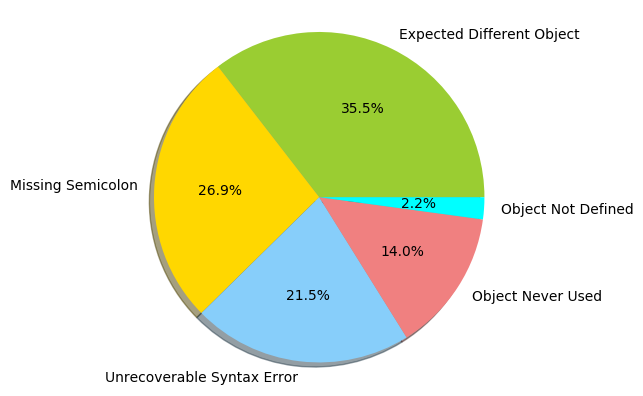
\includegraphics[width=\textwidth, keepaspectratio]{images/MCE2-npmchar.png}
	\caption{Δεύτερο συνηθέστερο λάθος των αρχείων του \en{char-rnn}}
	\label{MCE2-npmchar}
\end{figure}

\begin{figure}
	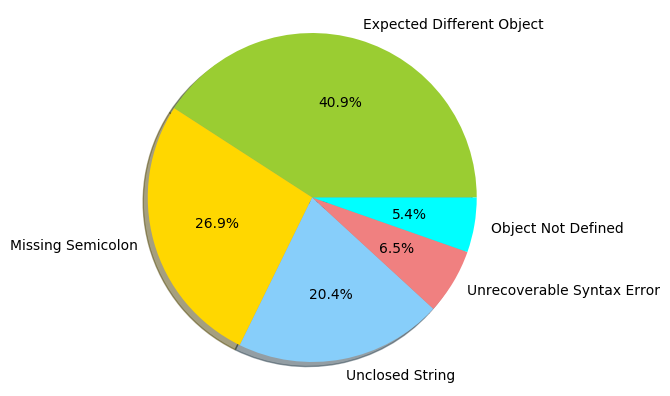
\includegraphics[width=\textwidth, keepaspectratio]{images/MCE-npmlabeled.png}
	\caption{Συνηθέστερο λάθος των αρχείων του \en{labeled-char-rnn}}
	\label{MCE1-npmlabeled}
\end{figure}

\begin{figure}
	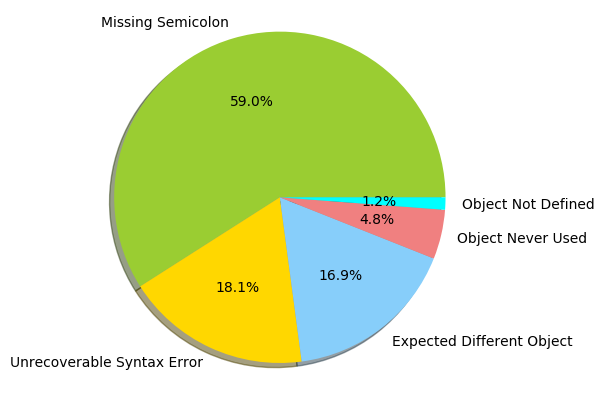
\includegraphics[width=\textwidth, keepaspectratio]{images/MCE2-npmlabeled.png}
	\caption{Δεύτερο συνηθέστερο λάθος των αρχείων του \en{labeled-char-rnn}}
	\label{MCE2-npmlabeled}
\end{figure}

\pagebreak 

\subsection{Παραγόμενος Κώδικας στα 100 δημοφιλέστερα \en{Github JavaScript Projects} με ρυθμισμένη δειγματοληψία}

Η μέθοδος παραγωγής κώδικα βασίζεται στη δειγματοληψία της εξόδου του συστήματος μας. Με σκοπό τη διερεύνηση της λειτουργίας των δύο μοντέλων, θα ρυθμίσουμε την κατανομή πιθανότητας που προτείνει το μοντέλο, ώστε να είναι πιο σίγουρο για τις προβλέψεις του. Χρησιμοποιούμε την συνάρτηση \en{Softmax Temperature} και επιλεγμένη τιμή για τη θερμοκρασία  0.85. Επιλέγουμε τα μοντέλα που εκπαιδεύτηκαν στο \en{Github js dataset} και τον ίδιο κώδικα αρχικοποίησης που χρησιμοποιήσαμε παραπάνω. Οι κώδικες 5.7, 5.8 περιέχουν αρχεία που παρήχθησαν από τα 2 μοντέλα. Στο κόστος της ποικιλίας του παραγόμενου κώδικα, τα μοντέλα κάνουν πιο <<συνηθισμένες>> επιλογές.   

\selectlanguage{english}
\lstinputlisting[language=JavaScript, caption={\tg{Δείγμα κώδικα από το }\en{char-rnn}\tg{ με ρυθμισμένη δειγματοληψία}}]{code/temp-char.js}
\selectlanguage{greek}

\pagebreak

\selectlanguage{english}
\lstinputlisting[language=JavaScript, caption={\tg{Δείγμα κώδικα απο το }\en{labeled-char-rnn}\tg{ με ρυθμισμένη δειγματοληψία}}]{code/temp-labeled-char.js}
\selectlanguage{greek}

Στις εικόνες \ref{static-temp-char} - \ref{MCE2-temp-labeled} παρατίθενται τα αποτελέσματα της ανάλυσης.
Το μέσο μήκος των παραγόμενων αρχείων ανεβαίνει σημαντικά σε σχέση με τις προηγούμενες προσεγγίσεις (218 γραμμές \en{char-rnn} -- 132 γραμμές \en{labeled-char-rnn}).
Όπως και στα προηγούμενα αποτελέσματα, το μοντέλο \en{labeled-char-rnn} κλείνει με μεγαλύτερη συνέπεια τα αρχεία του, αλλά τα παραγόμενα αρχεία ολοκληρώνουν σε μικρότερο ποσοστό τον συντακτικό έλεγχο επιτυχημένα.
Ενδιαφέρουσα είναι η εμφάνιση του λάθους \en{Object Already Defined} στα πιο συνηθισμένα λάθη.
Πράγματι, τα αρχεία που παράγονται από τα μοντέλα, τα οποία έχουν μεγαλύτερη πεποίθηση για τις προβλέψεις τους, τείνουν να επαναλαμβάνουν διάφορες δομές.

\begin{figure}
	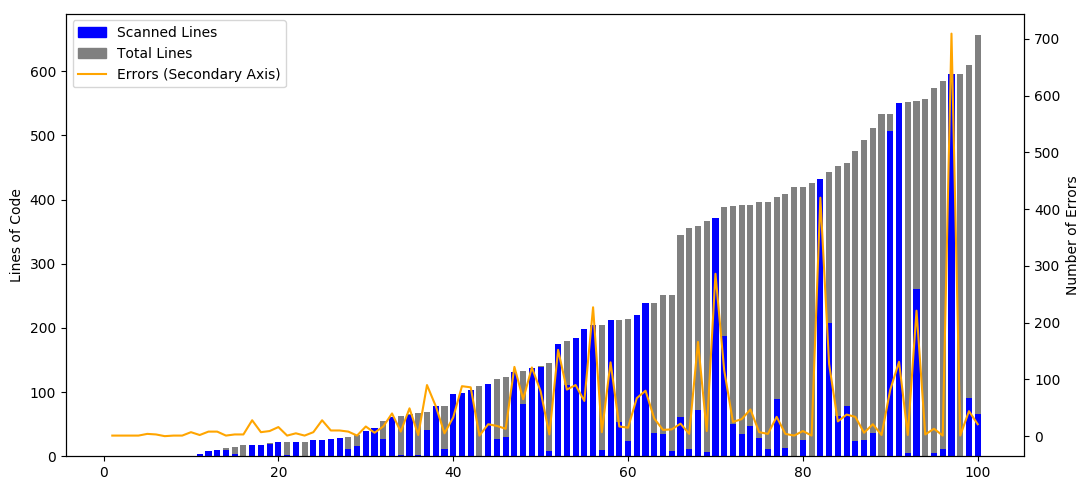
\includegraphics[width=\textwidth, keepaspectratio]{images/temp-char.png}
	\caption{Στατική ανάλυση κώδικα για τα αποτελέσματα του \en{char-rnn} μοντέλου}
	\label{static-temp-char}
\end{figure}

\begin{figure}
	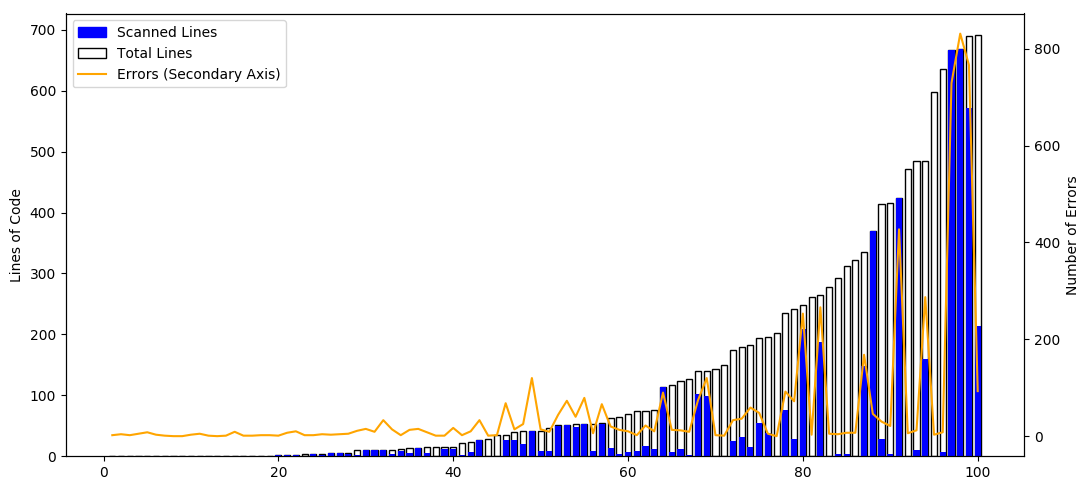
\includegraphics[width=\textwidth, keepaspectratio]{images/temp-labeled.png}
	\caption{Στατική ανάλυση κώδικα για τα αποτελέσματα του \en{labeled-char-rnn} μοντέλου}
	\label{static-temp-labeled}
\end{figure}

\begin{figure}
	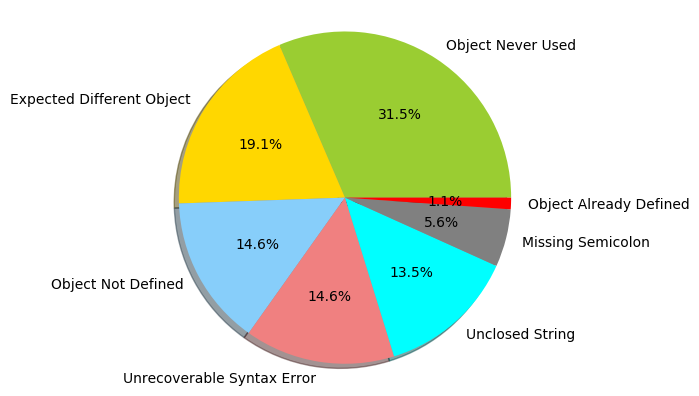
\includegraphics[width=\textwidth, keepaspectratio]{images/MCE-temp-char.png}
	\caption{Συνηθέστερο λάθος των αρχείων του \en{char-rnn}}
	\label{MCE-temp-char}
\end{figure}

\begin{figure}
	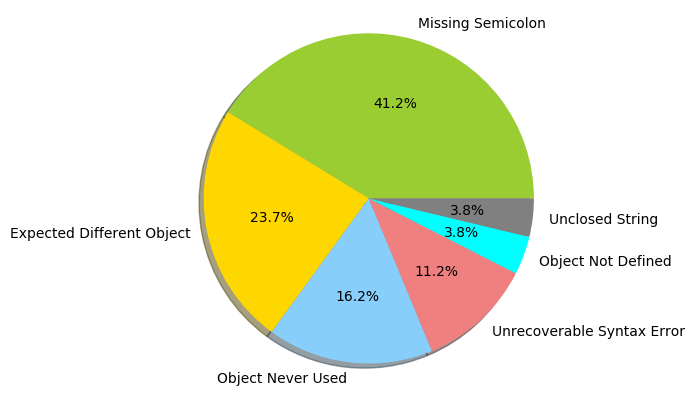
\includegraphics[width=\textwidth, keepaspectratio]{images/MCE2-temp-char.png}
	\caption{Δεύτερο συνηθέστερο λάθος των αρχείων του \en{char-rnn}}
	\label{MCE2-temp-char}
\end{figure}

\begin{figure}
	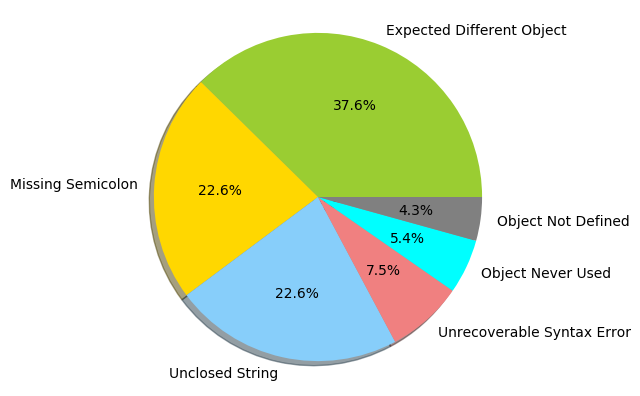
\includegraphics[width=\textwidth, keepaspectratio]{images/MCE-temp-labeled.png}
	\caption{Συνηθέστερο λάθος των αρχείων του \en{labeled-char-rnn}}
	\label{MCE2-temp-labeled}
\end{figure}

\begin{figure}
	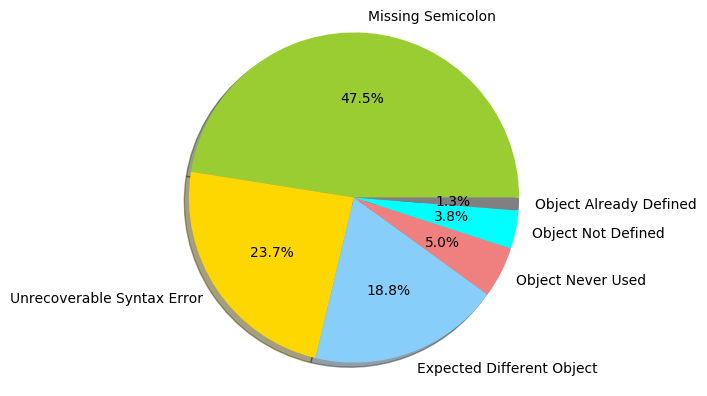
\includegraphics[width=\textwidth, keepaspectratio]{images/MCE2-temp-labeled.png}
	\caption{Δεύτερο συνηθέστερο λάθος των αρχείων του \en{labeled-char-rnn}}
	\label{MCE2-temp-labeled}
\end{figure}

\pagebreak

\subsection{Σχόλια περί σύγκρισης}

Τα αποτελέσματα της παραγωγής κώδικα που δεν είναι πραγματικά λειτουργικός είναι δύσκολο να ποσοτικοποιηθούν. Η εγγενής δυσκολία ερμήνευσης της εκμάθησης των νευρωνικών δικτύων, δυσκολεύει περαιτέρω την προσπάθεια αυτή. Με σκοπό την αποσαφήνιση των αποτελεσμάτων, δημιουργούμε μία απλή μετρική ώστε να συγκρίνουμε τα 6 μοντέλα που δοκιμάστηκαν.

\begin{ceqn}
\begin{align}
M = Errors_{avg} / (Lines_{avg} * \%Scanned_{avg})
\label{eq:M}
\end{align}
\end{ceqn}

\begin{table}[!h]
\centering
\caption{Τιμές της Μετρικής $M$ (Μικρότερες τιμές του $M$ είναι προτιμότερες)}
\begin{tabularx}{\textwidth}{|X|X|X|}
\hline
                    & \en{char-rnn} & \en{labeled-char-rnn} \\
\hline
\en{Github}       & 0.61             & 0.86                     \\
\hline
\en{NPM}       & 0.64             & 0.77                  \\
\hline
\en{Github Temperature}       & 0.38             & 0.52                  \\
\hline
\end{tabularx}
\label{Mtable}
\end{table}

Στη σχέση \ref{eq:M} $Errors_{avg}$ είναι ο μέσος όρος λαθών των αρχείων, $Lines_{avg}$ είναι ο μέσος όρος γραμμών των αρχείων και $\%Scanned_{avg}$ o μέσος όρος του ποσοστού ολοκλήρωσης συντακτικής ανάλυσης των αρχείων. Από τον πίνακα \ref{Mtable} μπορούμε να εξάγουμε 2 σημαντικές παρατηρήσεις.
Η πρώτη είναι πως το μοντέλο \en{labeled-char-rnn} έχει σταθερά χειρότερες επιδόσεις στην παραγωγή ποιοτικού κώδικα, παρόλο που έχει στη διάθεση του παραπάνω πληροφορία για τον κώδικα και μάλιστα σημαντική. Αυτό οφείλεται εν μέρει στην ταυτόχρονη στοχαστική επιλογή χαρακτήρα και είδους του, που μπορεί να επινοεί συνδυασμούς που δεν έχει ξαναδεί. Κατά δεύτερο λόγο, η στοχαστικότητα που εισάγεται για την παραγωγή κώδικα δυσκολεύει γενικότερα τα μοντέλα να γράψουν ορθά προγράμματα, για αυτό και όταν επιβάλλουμε στα συστήματα να εμπιστεύονται τις προβλέψεις τους, παίρνουμε καλύτερες τιμές για τη μετρική $M$.